% https://de.overleaf.com/learn/latex/How_to_Write_a_Thesis_in_LaTeX_(Part_1)%3A_Basic_Structure
% https://en.wikibooks.org/wiki/LaTeX/Document_Structure
%\documentclass[11pt, twoside]{report}
\documentclass[11pt, a4paper]{report}
%\documentclass[a4paper,11pt]{scrartcl}
\usepackage{syntonly}
%\syntaxonly
\usepackage[utf8]{inputenc}
\usepackage[backend=biber]{biblatex}
\addbibresource{mybib.bib}
\usepackage{hyperref}
\usepackage{graphicx}
\usepackage{color}
\usepackage{framed}
\usepackage{subcaption}
\usepackage{float}
\graphicspath{ {images/} }
\usepackage{blindtext}
\usepackage{mathtools}
\usepackage{amssymb}
\usepackage{amsbsy}
\usepackage{amsfonts}
\usepackage{amsthm}
\usepackage{amsmath}
\usepackage{IEEEtrantools}
%\usepackage{showframe}
%\usepackage[a4paper, width=150mm, top=5mm, bottom=5mm]{geometry}
\usepackage[a4paper, width=150mm, top=25mm, bottom=25mm]{geometry}
\usepackage{fancyhdr}
%\setlength{\headheight}{12pt}
%\setlength{\headheight}{15.2pt}
%\pagestyle{empty}
%\pagestyle{myheadings}
%\pagestyle{headings}
%\pagestyle{plain}
\pagestyle{fancy}
\fancyhf{}
%\fancyhead[L]{\leftmark:}
%\fancyhead[L]{\chapter~\thechapter:}
%\fancyhead[L]{\thechapter}
\fancyhead[C]{\rightmark}
%\fancyhead[R]{\thesection}
\fancyfoot[C]{\thepage}

\setlength{\parskip}{1.0em}
\setlength{\parindent}{1em}

\usepackage{lipsum}

\theoremstyle{plain}
\newtheorem{theorem}{Theorem}[chapter]
\newtheorem{lemma}[theorem]{Lemma}

\theoremstyle{definition}
\newtheorem{mydef}{Definition}[chapter]

\theoremstyle{remark}
\newtheorem{remark}{Remark}[chapter]


%newcommands
\newcommand{\N}{\mathbb{N}}
\newcommand{\C}{\mathbb{C}}
\newcommand{\R}{\mathbb{R}}
%\newcommand{\Z}{\mathbb{Z}}
\newcommand{\F}{\mathbb{F}}
\newcommand{\E}{\mathbf{E}}
\newcommand{\X}{\mathbf{X}}
\newcommand{\x}{\mathbf{x}}
\newcommand{\Z}{\mathbf{Z}}
\newcommand{\z}{\mathbf{z}}
\newcommand{\Y}{\mathbf{Y}}
\newcommand{\y}{\mathbf{y}}
\newcommand{\W}{\mathbf{W}}
\newcommand{\w}{\mathbf{w}}
\newcommand{\LL}{\mathcal{L}}
\newcommand{\NN}{\mathcal{N}}
%\newcommand{\B}{\{-1,1\}}
%\newcommand{\bvec}[1]{\mathbf{#1}}
%\newcommand{\bv}[1]{\mathbf{#1}}
%\newcommand{\b}[1]{\boldsymbol{#1}}
\newcommand{\bv}[1]{\boldsymbol{#1}}
\newcommand{\bvec}[1]{\boldsymbol{#1}}
\newcommand{\ceil}[1]{\lceil{#1}\rceil}
\newcommand{\floor}[1]{\lfloor{#1}\rfloor}
\newcommand{\gt}{>}
\newcommand{\lt}{<}
\newcommand{\tuple}[1]{\langle #1 \rangle}

\begin{document}
%\pagestyle{fancy}
\begin{titlepage}
\begin{center}
{
\includegraphics{images/MPIMG_RGB_gruen.png}}\\
\vspace*{1cm}
%\vfill
\Large
\textbf{List of topics to cover}
%\vfill

%\vspace{0.5cm}


%\normalsize
\large
With section titles and brief explantions.
\vfill
%\vspace{1.0cm}

Yiftach Kolb

Berlin, \today

\vfill
{
\includegraphics{images/fu-logo_bildschirm_RGB1.jpg}}
\end{center}
\end{titlepage}

%\author{Kolb, Yiftach}
%\date{Berlin, \today}
%\title{Topic List}
%\maketitle

\chapter*{Abstract}
punkt.
punkt.
\nocite{guo2017improved}

\chapter*{Declaration}
punkt.
punkt.
\nocite{bishop2006pattern}
\nocite{serre2001matrices}
\nocite{kingma2013auto}
\nocite{lotfollahi2018generative}

\chapter*{Acknowledgement}
punkt.\cite{kingma2013auto}
punkt.
bip/bop\slash boop
$\X \x \Z \z \Y \y \W \w \mathbb{Z}$
so-so--so---so

\listoftables

\listoffigures

\tableofcontents

\chapter{Introduction} punkt. \emph{punkt}, \textit{punkt}.

\chapter{Notations and definitions, preliminary concepts}
%\section{Basic Definitions}

\section{Basic notations}
\subsection{Vectors, matrices and tensors}
Throughout this paper (modulo typing errors) we use
capital bold math Latin or Greek letters ($\bv{X, \Sigma}$) to represent
matrices. To stress that we talk about matrices rather than vectors we show
product ($\times$) in the dimension, i.e $\bv{X} \in \R^{m \times n}$. Although
technically the matrix--space is the tensor product $\R^m \otimes \R^n$.

Bold small math letters ($\bv{x}$) represent usually row vectors, but in cases
where it makes sense may also represent matrices such as a batch of several
vectors (each row is a different data point). In few occasions it makes sense to
let it represent both a matrix and a vector, for example, $\bv{\sigma}$ may
represent both the covariance matrix and the variance vector of a diagonal
Gaussian distribution. Non-bold math letters ($x, \sigma$, \dots) may represent
scalar or vectors in some cases and hopefully it is clear from the context or
explicitly stated.

Since we are only dealing with real matrices the transpose and the conjugation
operators are the same ($A^T = A^*$) but over $\C$ conjugation is
usually the "natural" operation and we use it to indicate that some property is
still valid over $\C$ with conjugation.

Sometimes matrices are given in row/column/block notations inside brackets where
the elements are concatenated in a way that makes positional sense.
For example
both $(\x,\y)$ and $(\x | \y)$ represent a matrix with 2 \textbf{columns}.

As mentioned usually just $\x$ means a column vector and $\x^T$ means a row
vector but sometimes in matrix notation $\x$ represents a row when it makes
sense.
We use \textbf{curly} brackets to indicate the \textbf{row} representations of a matrix.
For example $\{\x, \y\}$ represents a matrix whose \textbf{rows} are $\x$ and $\y$
(as row vectors), which alternatively could be represented as
$(\x, \y)^T$.

$(\X,\Y)$ represents
concatenation of two matrices which implicitly means they have the same number
of rows.

Zero--blocks are indicated with $0$ or are simply left as voids. For
example $ \left( \begin{array}{c c} \bv{A} & \bv{B} \\ \bv{0} & \bv{D}
\end{array} \right) $ represents block notation of an upper--triangular matrix.

\begin{mydef}
Let $\X = \{\x_1, \dots \x_m\} \in \R^{m \times n}$
be a matrix in \textbf{row} notation. Then its \emph{squared Frobenius norm} is
\begin{equation}
\label{def:frobnorm}
\|X\|_F^2 \triangleq \text{trace}(\X \X^*) 
= \sum_{i=1}^{m} \|\x_i\|^2_2 = \sum_{i=1}^m \sum_{j=1}^n x_{ij}^2
\end{equation}
\end{mydef}


\subsection{Functions and maps}
Functions are usually understood to be scalar, namely $f:\R^n \to \R$ while maps
are more general $g:\R^n \to \R^m$. When we say that a map (or function) $\phi
:\R^n \to \R^m$ is \emph{parameterized}, it means that implicitly has additional 
variables that we treat as parameters $\phi_{\w}(\x) = \phi(\x, \w)$ where $\x \in \R^n$
and $\w$ is the parameter set which we don't always specify its domain and we may not
always subscript $\phi$ with it.

In the context of neural networks, when we say \emph{linear} map, we actually mean an
\emph{affine} map.
An affine map $f(x_1 \dots x_n)$ can always as linear map with one extra variable 
which is held fixed $x_0 \equiv 1$: $f(x_0, \dots x_n) = b + a_1 x_1 + \dots a_n
x_n$. $b$ is called the \emph{bias} of the map.
\label{affinelinear}

\section{The data}
we assume that the input data unless otherwise stated is real-valued matrix.
Rows represent \emph{samples} and columns represent \emph{variables}. We assume
that each raw is a realisation of a random vector. If we have $N$ rows, then the
corresponding $N$ random vectors are assumed to be independent. So depending on
the context, when we say observation, or row, we may mean the actual observed
values, or to the random vector who was realized by said observation.

We deal with two type of concrete datasets in this thesis. One of them is
Single cell RNAseq data. This data represents gene expression levels in 
individual cells, where rows represent cells and columns represent genes.
So if we see a reading of
$0.5$ in row $2$ column $4$ in means that in cell $2$ gene $4$ has normalized
expression of $0.5$.

The other type of data is images. For example the MNIST data set contains 
greyscale $28 \times 28$ images of hand written digits.
We still think of such data set as a matrix. The first axis always represents
the samples, so each "row" represent an image. The rest of the axes represent
the image. Alternatively we can also flatten the images into one axis and think
of an image as a row vector of $28*28$ dimensions.

There could possibly be additional data matrices with information about
class or conditions. We use \emph{one-hot encoding} to represent such
information.
For example in the case of the MNIST dataset every image also comes with a label
which indicate which digit it shows. Since there are $10$ classes of digits ($0$
to $9$) the class matrix is going to have $10$ columns and each row is a one-hot
vector indicating the digit of the correspoinding image.

\begin{mydef}
\label{def:datamatrix}
A \emph{data matrix} is a real--valued matrix $\bv{X} \in \R^{N \times n}$
which represent a set of $N$ $n$-dimensional data points.
The $N$ rows are also called \emph{observations} and the $n$ columns are
\emph{variables}.
\end{mydef}

\begin{mydef}
\label{def:classmatrix}
A \emph{class matrix}, or also a \emph{condition matrix}
$\bv{C} \in \R^{\N \times c}$ is simply a real matrix which
represents one-hot encoding of $c$ classes or conditions over $N$ samples.
For example if sample $i$ has class $j$, then 
$(\forall k\in 1, \dots, c) \bv{C}[i,k] = \delta_{jk}$.

We say that that $\bv{C}$ is a \emph{class probability matrix} or a \emph{relaxed
class matrix} (same with condition)
if instead of being one-hot it is a distribution matrix, namely each row is
non-negative and sums up to $1$.
\end{mydef}

Usually if the input data includes class/condition information, it comes as a
class matrix (pure one-hot) but the output (the prediction) is naturally 
probabilistic and hence is relaxed.

\subsection{Input set and target set}
Sometimes the data paired into the input data $\X$ and the
target data $\Y$, 
representing for example, samples from some unknown function $f(\x) = \y$
that we want to "learn" to represent.
In classification tasks for example, $\X$ can be for example a set of images,
and $\Y$ can be their labels.

In the case of autoencoders, the target set is also the input set and $f$ is the
identity (in this case $f$ is known but we want to learn an efficient way
to represent the data).

When our data comes in several matrices, for example it could be a single cell RNAseq data
with normalized gene expression data $\X$,  and cell types as target
matrix $\Y$. It means they have must the same number of rows. And when we speak about 
paired input/target $\x,\y$ it means some $(\x,\y) \in (\X,\Y)$ so it should be
clear they belong to the same sample (row).

%\begin{mydef}
%\label{paired data}
%Let $\X = \{\x_i\}_1^N,\quad \Y = \{\y_i\}_1^N$ be two matrices in row noataion
%with the same number of rows $N$. Then
%\begin{equation}
%(\X,\Y) \triangleq \{(\x_i,\y_i)\}_1^N
%\end{equation}
%\end{mydef}


\section{Linear algebra preliminary: SVD and PCA}
In the following state some facts and bring without proof what are the singular
value decomposition and the principle components of a matrix. For a
full proof see~\cite{serre2001matrices}.

%\section{SVD and PCA}
Let $\bv{X} \in \R^{N \times n}$ be a real-valued matrix
representing $N$ samples of some
$n$-dimensional data points and let
$r= \text{rank}(\bv{X}) \leq \min(n,N)$. 

$\X \X^*$ and $\X^* \X$ are both symmetric and positive semi-definite.
Their eigenvalues are non-negative, and they both have
the same positive 
eigenvalues, exactly $r$ such, which we mark
$s_1^2 \geq s_2^2 \geq \dots s_r^2 \gt 0$. The values
$s_1 \dots s_r$ are called the \emph{singular values} of $\bv{X}$.

Let $\bv{S} = 
\begin{pmatrix}
s_1 & & &\\
& s_2 & &\\
& & \ddots &\\
& & & s_r
\end{pmatrix} \in \R^{r \times r}
$

Let $\bv{U} = (\bv{u}_1 | \dots | \bv{u}_N) \in \R^{N \times N}$
be the (column) right eigenvectors of $\X \X^*$ sorted
by their eigenvalues. 
Then $\bv{U} = (\bv{U}_r, \bv{U}_k)$ 
where $\bv{U}_r = (\bv{u}_1 | \dots | \bv{u}_r) \ \in \R^{N \times r}$ are the first $r$
eigenvectors corresponding to the non-zero eigenvalues, and $\bv{U}_k$ are the
eigenvectors corresponding to the $N-r$ $0$-eigenvalues.
Similarly let 
$\bv{V}  = (\bv{V}_r, \bv{V}_k)\in \R^{n \times n}$
be the (column) right eigenvectors of $\X^* \X$, sorted
by the eigenvalues, 
where $\bv{V}_r  = (\bv{v}_1 | \dots | \bv{v}_r) \in \R^{n \times r}$ are the firs $r$
eigenvalues and $\bv{V}_k$ are the $n-r$ null-eigenvectors.

The critical observations is that $\bv{V}_r = \bv{X}^* \bv{U}_r S^{-1}$
and then $\bv{U}_r^* \X \bv{V}_r = S$.

The \textit{singular value decomposition (SVD)} of $\X$ is 

\begin{equation}
\label{eq:svd}
\X = \bv{U} \bv{D} \bv{V}^*
\end{equation}
where 
$\bv{D} =
\left(
\begin{array}{c c}
\bv{S} & \bv{0} \\
%\hline
\bv{0} & \bv{0}
\end{array}
\right) \in \R^{N \times n}
$ is diagonal.

$\bv{V}_r$ are called the \textit{(right) principal components} of $\X$.
Note that $\bv{V}_r^* \bv{V}_r = \bv{I}_r$ and that 
$\X = \X \bv{V}_r \bv{V}_r^* = (\X \bv{V}_r) \bv{V}_r^T$. If one looks at the second expression, 
it means that the each row of $\X$ is spanned by the orthogonal
basis $\bv{V}_r^T$ (because the other vectors of $\bv{V}$ are in $\text{ker}(\X)$.

More generally
For every $l \leq r$, let $\bv{V}_l \in \R^{N \times l}$ be the first $l$ components,
Then $\X\bv{V}_l \bv{V}_l^T$ is as close as we can get to $\X$ within an
$l$-dimensional subspace of $R^n$, and $\bv{V_l}$ minimizes

\begin{equation}
\label{eqn:pca}
\bv{V}_l = \text{argmin}_{\W} \{
\|\X - \X \bv{W}\bv{W}^T\|_F^2 \quad : \quad \bv{W} \in \R^{n \times l}, \bv{W}^T \bv{W} =
\bv{I}_l\}
\end{equation} 

Where $\| \cdot \|_F^2$ is simply the sum of squares of the matrix' entries.

If we consider the more general
minimization problems: 

%\begin{subequations}
\begin{IEEEeqnarray}{C}
\label{eqn:pca2}
%\begin{aligned}
\min_{\bv{E,D}}\{\|\X - \X \bv{E}\bv{D}\|_F^2 \quad : 
\quad \bv{E,D^T} \in \R^{n \times
l},\} \\
\label{eqn:pca3}
\min_{\W}\{\|\X - \X \bv{W}\bv{W}^{\dagger}\|_F^2 \quad : 
\quad \bv{W} \in \R^{n \times
l},\}
%\end{aligned}
\end{IEEEeqnarray}
%\end{subequations} 

It can be shown~\cite{plaut2018principal} that the 
last two problems~\ref{eqn:pca2},~\ref{eqn:pca3} are equivalent
and that for any solution $E,D$ it must hold that 
$\bv{D}=\bv{E}^{\dagger}$. ($\bv{D}$ is the Moore--Penrose generalized
inverse of $\bv{E}$).
Moreover,
$\bv{V}_l$ still minimizes the general problem~\ref{eqn:pca2} and for every
solution $\bv{W}$, it must hold that $\text{span}\{\bv{W}\} =
\text{span}\{\bv{V}_l\}$ (but it isn't necessarily an orthogonal matrix).

\section{Neural networks}

We briefly discuss here some of the basics of neural network to provide clarity
and motivation. Mostly based on~\cite{nielsen2015neural}.

\subsection{Universal families of parameterized maps}
If we take an expression such as $f_{a,b}(x) = ax + b$, if we hold $(a,b)$ fixed
on specific values, then we get a linear function on $x$. Every assignment of
$(a,b)$ defines a different linear function and in fact every linear function on
one dimension can be uniquely described by these $a$ and $b$. So we can say that
$\{f_{a,b}\}_{a,b \in \R}$ is a \emph{parameterization} of the class of all real
linear functions on one variable. The distinction between what are the variables and what are
the parameters is somewhat arbitrary
and in the end, $f_{a,b}(x)$ is just another way to represent 
a $3$-variable function $f(a,b,x)$. 

In general we can define one or more multivariate
functions $g : \R^{n+m} \to \R^k$ (for simplicity of the discussion lets assume 
it is defined everywhere) and partition the set of its variables into $2$. 
$g_{\w}(x) \triangleq g(\w,\x)$ where 
$\x \in \R^n, \w
\in \R^m$ and let $g_{\w}(\x) := g(w,x) \in \R^k$.


We call a class $\mathcal{F}$ of parameterized functions \emph{universal} if
every continuous function can be uniformly approximated (inside a bounded
domain) by functions of that class. The class of all linear functions is not
universal. But taking "any function" $g$ is too general. What we actually want
is a class of parameterized functions that is:
\begin{itemize}
\item{} as simple as possible to construct
\item{} derivable in both the parameters as well as the variables
\item{} can uniformly approximate any continuous function in a bounded domain
given sufficiently large set of
parameters (i.e. is universal).
\end{itemize}

However these requirements are still not enough.
For example, the class of multivariate polynomials can
uniformly approximate any function. However it may not be a good idea to try
to learn very complicated high dimensional data using polynomial representation. 
For one reason is that the number of terms (monomials) grows very rapidly with the
dimension and the degree of the polynomials: for $n$ dimensions and $m$ degrees
there are something like $\binom{m + n}{n}$ monomial terms.

We want this class of simpler functions, that are almost as simple as linear,
and yet that suits well for statistical learning. For example we want to
represent complicated functions with relatively few parameters.

One such class of functions is the feed forward neural networks,
which is the class of functions that are comprised from "neurons".

\subsection{Neurons}

So what a "neuron"?. 
Inspired from biology, a \emph{neuron} is a many to one ($\R^n \to \R$) parameterized
function which
"integrates" the input with a linear, or affine~(see~remark~\ref{affinelinear})
function, and 
then applies a non-linear scalar function, which we call an \emph{activation
function}.
In a sense it is the simplest
function that is not linear.
Moreover we only need one type of non-linear activation, e.g sigmoid, to
construct arbitrarily complex neural networks.
A degree 2 polynomial would be considered "less 
simple" because it applies multiple non-linear multi-variable
functions $x_i x_j\dots$.

\begin{mydef}
\label{def:activationfunction}
An \emph{activation function} $\sigma : \R \to \R$ is any one of the following functions:
$x \mapsto 1$ (constant), $x \mapsto x$ (identity)
$ x \mapsto \frac{e^x}{1 + e^x}$ (sigmoid), and $x \mapsto \max(0,x)$ (ReLU).

If $\x = (x_1, \dots x_n) \in \R^n$ then $\sigma(\x)$ is the element-wise application
$\sigma(\x) \triangleq (\sigma(x_1), \dots , \sigma(x_n))$.
\end{mydef}

In the official definition we narrowed it down to just 4 kinds but in general
there are plenty of other activation functions. Also note that these functions
have no parameters.

\begin{mydef}
\label{def:neuron}
Let $\sigma : \R -> \R$ be an activation function and let $f_{\w} : \R^n -> \R$
be a \emph{parameterized} linear function. A \emph{neuron} $\nu$ is the
parameterized function 
$\nu =  \nu_{\w} \triangleq \sigma \circ
f_{\w}$.
%In case that $n=0$ then $\w = \emptyset$, we let $\nu \triangleq \sigma$.

The parameters $\w$ are called the \emph{weights} of the neuron $\nu$.
\end{mydef}

Think of the weights of a neuron as some mutable, tunable property, some sort of memory.

\begin{figure}[!h]
\begin{framed}
\centering
\begin{subfigure}[b]{0.45\textwidth}
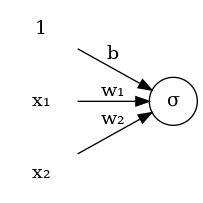
\includegraphics[width=0.4\textwidth]{./images/models/neuron.gv.png}
%\label{fig:neuron1}
\end{subfigure}
\begin{subfigure}[b]{0.45\textwidth}
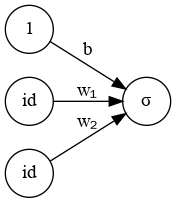
\includegraphics[width=0.4\textwidth]{./images/models/neuron.2.gv.png}
\end{subfigure}
\caption{Two graphical descriptions of the neuron
$\sigma(w_1x_1 + w_2x_2 + b)$}. Here the bias $b$ is explicitly shown
but usually it is not depicted. In the left the variable names are explicitly
shown, while in the right they are not.
\label{fig:neuron2}
\end{framed}
\end{figure}

Connecting many neurons together can create powerful parameterized
functions which we call neural networks.
Connecting means that the output of one neuron is the input to one of the
variables of a different neuron.
In feed forward networks the information only goes in one direction (no
feedback) and as we will see it means the network is a directed acyclic graph.

\begin{mydef}
\label{def:NN}
A \emph{feed forward neural network (NN)}is a \textbf{parameterized} map $\phi$
recursively defined
follows:
\begin{enumerate}
\item{} 
Activation functions ($1$, $id$, and $\sigma$) are NNs which are called the
\emph{elementary neurons} and they have no parameters ($\w=\emptyset$).
\item{} neurons are NNs
\item{} If $\psi :\R^n \to \R^m$ is a parameterized linear map then it is a NN.
\item{} If $\psi : R^n \to \R^m$
and $\rho: \R^m \to \R^l$ are NNs and their parameter sets are disjoint then $\phi = \rho
\circ \psi$ is a NN.
\item{} if $\nu:\R^n \to \R^m$ is a NN
and if $\psi_i: \R^{k_i} \to \R^{n_i}, i =1 \dots l$ are NNs, such that
$\sum_1^l n_i = n$
%and if $\psi_1, \dots \psi_n$ are NNs,
and if the parameter set of $\nu$ is disjoint from the combined parameters of
the $\psi_i$'s then
$\phi = \nu(\psi_1, \dots, \psi_n)$ is a NN
%if the dimensions "make sense".
.
\end{enumerate}

The parameter set $\w$ is called the \emph{weights} of $\phi$.
Often we don't distinguish between the network $\phi$ and its weights, and
we identify both as $\phi$.

In the definition we made the range and domain to be the entire $\R^n$ but
it is not necessary, we just need for the composition to be valid.
\end{mydef}

Feed forward neural network 
are depicted as a directed acyclic graph where every node (with its incoming
edges) corresponds to a neuron.
You can think of figure~\ref{fig:neuron2} left as depicting the neuron "component" 
in a network, while figure~\ref{fig:neuron2} right shows a neural network
description of single neuron, comprised from elementary neurons.
If we add more neurons and add depth to the

If rule 5 of the definition is not used in the construction of $\phi$, then the
resulting network is hierarchical. Its graph can be partitioned into \emph{levels}
$l_0, l_1\dots$ and there are only directed edges between two consecutive
levels $l_i \to l_{i+1}$ (see figure~\ref{fig:nn1}).

The label inside the neuron describes its activation function.
In the diagrams, we let $\sigma$ represent the sigmoid function.
We represent the identity function either by the name of the variable ($x_1$,
$y$ etc.) it acts on or simple by 
$id$.   We let the label $1$ represent the constant function. We need the
constant function because with it we can represent any affine map as a linear
map with the first input always clamped to $1$. But connecting $1$ to every
(non-input level) neuron would clutter the graph so it is not shown in most
diagrams but still implicitly assumed.
A directed edge between neurons means that the output of the neuron at the tail
is multiplied by the edge weight and assigned to the input variable of the
neuron it connects to.
Input-level neurons (sources) have no incoming edges and they represent the
beginning of the
computation.
Output neurons (sinks) have no outgoing edges and their output is the final result of
the computation.

A Node's output is therefore only dependent on the output of its direct
ancestral nodes 
(plus the bias which is usually not shown).

\begin{figure}[!h]
\begin{framed}
\centering
\begin{subfigure}[b]{0.5\textwidth}
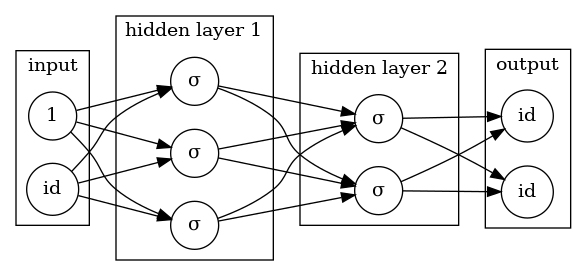
\includegraphics[width=0.8\textwidth]{./images/models/neuronlayers.gv.png}
\end{subfigure}
\begin{subfigure}[b]{0.5\textwidth}
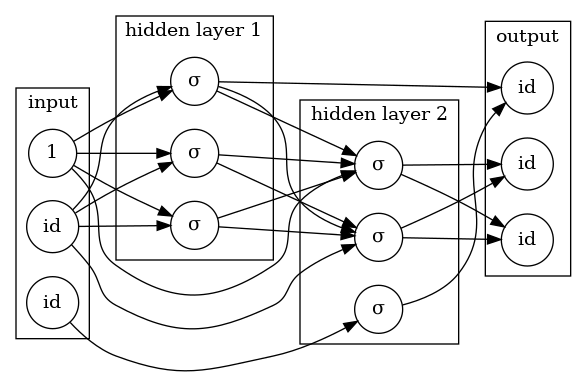
\includegraphics[width=0.8\textwidth]{./images/models/neuronlayers.2.gv.png}
\end{subfigure}
\caption{The network in the top didn't use rule 5~\ref{def:NN} in the construction.
It is strictly hierarchical and there are only edges between nodes of two
consecutive layers. The one on the bottom is more general.
}
\label{fig:nn1}
\end{framed}
\end{figure}


%\begin{figure}[!h]
%\centering
%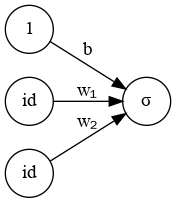
\includegraphics[width=0.3\textwidth]{./images/models/neuron.2.gv.png}
%\caption{a neural network graphical description
%$\sigma(w_1x + w_2y + b)$}
%\label{fig:neuron2}
%\end{figure}


It turns out~\cite{nielsen2015neural} that the feed forward neural networks
with a single type of non-linear activation (e.g. sigmoid) and a single hidden
layer
are "universal"; Which means that
any continuous function $f$ can be
uniformly approximated by a feed forward neural network
with a single hidden layer and Sigmoid as the non-linear
activation function.
More precisely, let $B \subseteq \R^n$ be a bounded domain. Let $f : B \to \R^m$
be continuous, and let $\epsilon \in (0,1)$. Then there is a feed forward neural
network with a single hidden layer $\phi = \phi_{\w}$ and there is some value assignment
for the parameters $\w$ such that 
$(\forall \x \in B) \|\phi(\x) - f(\x)\|_2 \lt \epsilon $. The size of that single
hidden layer (the number of parameters) depends on $f$ and $\epsilon$.

In the definitions we only used linear maps to grow the network. 
There are other types of maps which are used, most commonly are convolutions 
but the principles and the graphical description remain essentially the same.

There are additional types of parameterized functions which are used "within the
layer" such as batch normalization but we won't get into that as this is not a
thesis about neural networks per se.

\begin{figure}[!h]
\begin{framed}
\centering
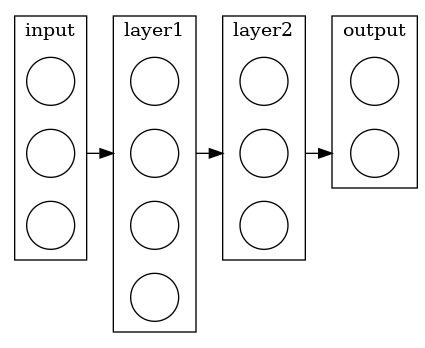
\includegraphics[width=0.5\textwidth]{./images/models/multilayer.gv.png}
\caption{
A graph of a hierarchical feed forward neural network where the connections 
are abstracted. Edges between layers may represent in this case a fully
connected layer (every neuron has incoming edges from all neurons of the
previous layer) but it could also be used for describing a convolution.
}
\label{fig:nn2}
\end{framed}
\end{figure}

As figure~\ref{fig:nn1} shows, 
The input layer is the where the input $(\x)$ is "fed in" and the output layer
is the final result of the evaluation $\phi(\x)$.
We call all the layers (or neurons) that are 
not in the input level or the output level "hidden"
because we don't usually know what is the input/output value in these.

\subsection{Loss functions}


In the claim about neural networks being "universal" in terms of approximating
function $f(\x)=\y$ with neural network $\phi(\x)$. We stated specifically
convergence in terms of $l_2$ norm
$\|\phi(\x) - \y \|_2$, but the claim holds in theory and in
practice with other types of "distance-like" functions which we call loss
functions.

Moreover we usually don't know what is the function $f$ which we try to
approximate. Rather we are given 
paired samples of input/target $(\x, \y)$ and we
try to minimize the total error.

\begin{mydef}
\label{def:lossfunc}
Let $\phi :\R^n \to \R^m$ be a neural network.
A \textit{loss function} is a differentiable
function $\mathcal{L} : \R^{m+m} \to \R$. 
With "distance-like quality".
\end{mydef}

Typically the loss function is additive on the dimension, meaning it has the
form $(\forall \y,\z \in \R^m) \mathcal{L}(\y, \z)) = \sum_{i=1}^m \psi(y_i,
z_i))$

Let $\X \in \R^{N \times n}, \Y \in \R^{N \times m}$ be the input and the target
set and let $(\x,\y)$ be a paired input/target. 
We use the loss function $\mathcal{L}$ as the target function for 
the minimization problem,
 $\min_{\w} \sum_{(\x,\y)}\mathcal{L}(\phi(\x), \y)$ where the sum goes over all
paires ($N$ rows)  (input, target).


For example
$\mathcal{L}(\y, \z)) = \|\y - \z\|_2^2 = 
\sum_i |y_i - z_i|^2$ is a one such loss function (the
square error).

So far we defined $\phi$ and $\mathcal{L}$ on single input/target data points
$\x$ and $\y$. But we are interested in minimizing the total error
$\mathcal{L}(\phi(\X),\Y)$. So first we need to state how these functions
operate on sets of samples (matrices) rather than on data points (vectors).

Usually evaluation over the entire dataset is infeasible. Instead computation is
performed on batches, which are relatively small chunks of the data.

\begin{mydef}
\label{def:batch}
Let $\bv{X} \in  \R^{N \times n}$ be a data matrix. A \emph{batch}
$\bv{x} \in \R^{b \times n}$ is any subset of $b$ rows of $\bv{X}$
(Note that in this case $\x$ represents a matrix).
\end{mydef}

Batch $\x = \{\x_1, \dots \x_b\} \in \R^{b \times n}$ (row notation)
represents a subset of $b$ samples out of the total of $N$ samples in the
dataset.
Extending $\phi$ to operate on batches is trivial.
$\phi(\x) = \{\phi(\x_i)\}$ is the matrix where $\phi$ is applied on the rows of the bath.
Given an input batch $\x$ and corresponding target batch of $\y$,
We extend the loss function to batches by averaging over the batch:
$\mathcal{L}(\phi(\x), \y) \triangleq \frac{1}{b} 
\sum_{i=1}^b \mathcal{L}(\phi(\x_i), \y_i)
$

\begin{mydef}
Let $\phi$ be a neural network as defined in~\ref{def:NN} and let $\mathcal{L}$
its associated loss function as defined in~\ref{def:lossfunc}---over vectors.
Let $\x = \{\x_1, \dots , \x_b\} \in \R^{b \times n}$ be a $b$-batch (in row
notation)
, and let $\y = \{\y_1, \dots , \y_b\} \in \R^{b \times m}$ be a corresponding
target batch.
Then $\phi$ and $\mathcal{L}$ \emph{extended} over batches are:
\begin{IEEEeqnarray}{C}
\phi(\bv{x}) \triangleq \{\phi(\bv{x}_i)\}_{i=1}^m \in \R^{b \times m}\\
\label{eq:NNbatch}
\mathcal{L}(\phi(\x), \y) \triangleq \frac{1}{b}\sum_{i=1}^b \mathcal{L}(\phi(\x_i), \y_i) \in \R
\label{eq:NNbatchloss}
\end{IEEEeqnarray}
\end{mydef}

If $\mathcal{L}$ is the square error function $\| \cdot \|_2^2$ on vectors,
then its extension to batches is $\frac{1}{b}\| \cdot \|_F^2$. The reason why we
sum and don't average over the dimensions will be cleared later when we get into
variational inference.

There is also a probabilistic way to interpret the total loss.
We assume that the data points $\X, \Y$ were randomly sampled from the unknown
data distribution $P(\x, \y)$.
Then equation~\ref{eq:NNbatchloss} can be reformulated as the expected 
loss~\cite{bishop2006pattern}:

\begin{equation}
\mathcal{L}(\phi(\x), \y) \approx
\mathrm{E}_{\x,\y \sim P(\x,\y)} \mathcal{L}(\phi(\x), \y)
\label{eq:NNbatchlossE}
\end{equation}

\subsection{Training}
This is just a brief explanation of the basic principals. Training deep networks
is a big subject which has many challenges and obstacles and a lot of
heuristics are used. 

Training the neural network $\phi_w$ means finding the weights that minimize the
loss function applied on the training input/target paired sets $\X,\Y$, in other
words minimizing $\min_{w} (\mathcal{L}(\phi_w(\X),\Y)$.
Usually we can't compute efficiently $\phi$ and $\mathcal{L}$ over the entire
sets because $N$ is too large, therefore we use batches.

\begin{mydef}
Let $\phi_{\omega}$ be a neural network and $\mathcal{L}$ its associated loss
function. And let $(\X, \Y)$ be our \emph{training set} consisting of 
the data matrix $\X$ and $\Y$
the corresponding target matrix.
Then \emph{Training} of $\phi_{\omega}$ with respect to $\mathcal{L}, \X$ 
means
algorithmically approximating the minimization problem:
\begin{equation}
\label{def:training}
\min_{\omega} \mathcal{L}(\phi_{\omega}(\X), \Y)
\end{equation}
\end{mydef}

During a \emph{training step} the network is applied on a batch $(\x,\y)$. Then the
loss function is applied on the output of the network and a gradient (with relation to the
weights) is taken using the efficient backpropagation
algorithm~\cite{nielsen2015neural}.
The gradient is used for the weight update rule, which
varies depending on the specific training algorithm. Typical training algorithms
are SGD (stochastic gradient decent) and Adam~\cite{jais2019adam},
which is the one used throughout
this work.

We only need to define the network, the loss function and the specific training
algorithm. The rest (derivation, weight update etc.) is taken care for us by the
backend of the software (Pytorch~\cite{pytorch2018pytorch}) and can be regarded
as a black box.

\section{Autoencoders}

The basic type of an autoencoder which we informally call "vanilla" autoencoder
is a neural network that tries to "learn" the identity function. Though it sounds
pointless on a first thought, the point is how we construct this network. An
autoencoder consists of two neural networks.
An encoder network maps the input into a lower dimensional so called "latent
space", and a decoder network maps the latent space back into the high
dimensional input layer.
In the case of the vanilla autoencoder the target for the loss function is the
same as the input $\Y = \X$.

\begin{figure}[!h]
\begin{framed}
\centering
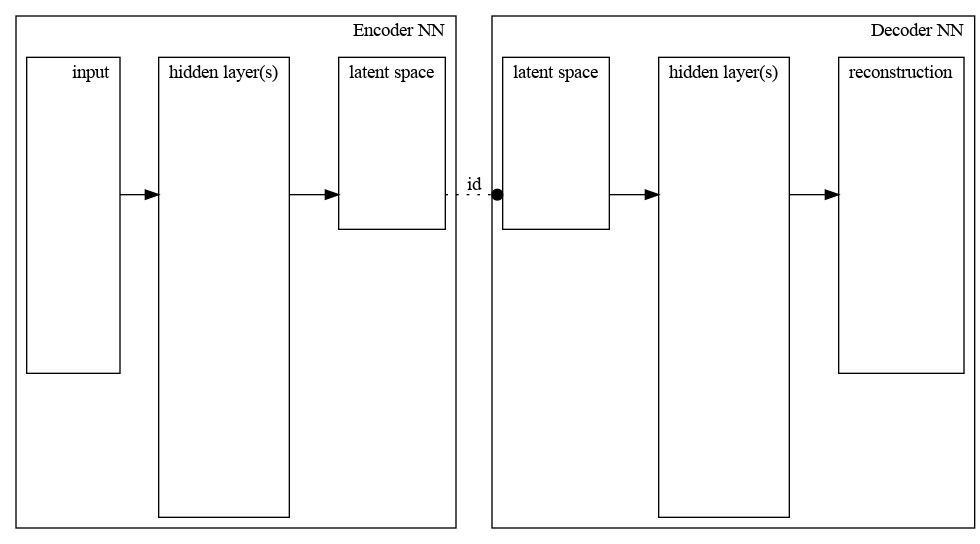
\includegraphics[width=0.8\textwidth]{./images/models/autoencoderNN.gv.png}
\caption{
A graphic description of a "vanilla" autoencoder.
}
\label{fig:autoencoder}
\end{framed}
\end{figure}

\begin{mydef}
\label{def:autoencoder}
An \textit{Autoencoder} (AE) is a pair 
$(\phi, \psi)$ of feed forward neural networks 
$\psi : \R^n \to \R^m, \nu : \R^m \to \R^n$.

$\psi$ is called the \emph{encoder} network, and $\nu$ is called the
\emph{decoder} network and the composition
$\phi = \nu \circ \psi$ is called the \emph{autoencoding network}. 

We call $\R^m$ or more genrally the domain of the decoder, \emph{the latent
space}, and $\R^n$ (or more generally the domain of the encoder) is called
\emph{the observed space}.

Given a batch $\x \in \R^{b \times n}$ we call $\z = \psi(\x) \in \R^{b \times m}$
the \emph{latent representation} of $\x$ or the \emph{encoding} of $\x$.
\end{mydef}

While the definition as is given is symmetric, it is assumed that $n > m$, and
therefore $\psi$ represents dimensional reduction (in other words encoding) of
the data and $\nu$ represents expansion back to original space (decoding).

The idea here is that the original high dimensional data can be embedded
in a low dimensional space by the encoder. The decoder then can reconstruct the
original data from the embedding.

%A typical loss function for the AE is usually the mean sum of squares (MSE)
%$\mathcal{L}(X;\phi) = \frac{1}{N}\|X - \phi(X)\|_F^2 = \frac{1}{N}\|X - D \circ
%E (X) \|_F^2$.

%Note that the MSE can be interpreted probabilitically, if we assume our input
%comes from a random diagonal Gaussian with constant unit variant, we can interpret
%$D(E(X)) = \mu_x$ and the mean square error is $\log \mathcal{N}(x ; mu_x, 1)$
%(up to some scaling factor). Where $\log \mathcal{N}(\cdot ; \mu_x, 1)$ is the 
%log-density function for diagonal Gaussian with mean $\mu_x$ and unit variance. 

\subsection{Relation between PCA and AE}
For \textbf{centered} data, meaning every variable (column of $\bv{X}$)
has a sample mean of $0$, the first $k \leq \text{rank}(\bv{X})$ principle components
$\bv{P}$ are the solution for equation~\ref{eqn:pca}; Whereas a \textbf{linear}
autoencoder solves equation~\ref{eqn:pca3}. As mentioned, it must hold that $E =
D^{\dagger}$ (the encoder must be the Moore-Penrose inverse of the decoder).

A linear autoencoder (an AE where $\phi$ is linear) is therefore almost equivalent to
PCA~\cite{plaut2018principal}, in that in the optimum, a bottleneck space of dimension $k$
is spanned by the first $k$ principle components of the input $\bv{X}$.
In general, an AE can be seen a PCA-like, but non-linear method for
dimensionality reduction.

\chapter{Variance inference and variational autoencoders}
\section{Variational Inference}

Here we briefly explain the idea behind variational inference and introduce the
ELBO which is the loss function we'll use throughout this text.
For more details see~\fullcite{bishop2006pattern}.

We treat the data matrix as a set of independent observations (its rows)
$\bv{X} = \{\bv{x}_1, \dots
, \bv{x}_N\}$ which we try to explain by a probabilistic model. 
Each row $\x_i$ is thought of a realization of a random vector, which we also 
denote as $\x_i$ (as explained in the notation section) and similarly $\X$
represent both the set of r.vs as well as the realization itself.
We assume that
the $\bv{x}_i$'s are independent and identically distributes (i.i.d) random vectors
with some distribution function $p(\x)$ and therefore for
the entire dataset it holds that $p(\bv{X}) = \prod p(\bv{x}_i)$.

\begin{mydef}
\label{def:logevidence}
Let $\bv{X} \in \R^{N \times n}$ be a data matrix and let $\{\bv{x}_i\}_1^n$ be its
rows,
which we assume to be i.i.d with some (unknown) distribution $p(\bv{x})$.
Then $\log p(\bv{X}) = \sum_1^N \log p(\bv{x}_i)$ is called the \emph{log evidence} of our
data.
\end{mydef}

The r.vs $\bv{X}$ are high dimensional however
we have some reason to believe that behind the scenes there are some hidden
(latent), smaller dimensional, r.vs
$\bv{Z} = \{\bv{z}_1 \dots \bv{z}_N\}$ that generate the observations $\bv{X}$.
In other words we think that $\bv{X}$ is conditioned on $\bv{Z}$ and we can speak of
the joint distribution $p(\bv{X},\bv{Z}) = p(\bv{X}|\bv{Z})p(\bv{Z})$.
Because we assume i.i.d for both $\bv{X}$ and $\bv{Z}$ all the distributions factor
over the individual samples multiplicatively, e.g.
$p(\bv{X}|\bv{Z}) = \prod p(\bv{x}_i | \bv{z}_i)$,
$p(\bv{X}) = \prod p(\bv{x}_i)$ and so forth. This makes working with log
probabilities very easy.

Suppose that we have a fully Bayesian model. In this case there are no
parameters because the parameters are themselves stochastic variables with some
suitable priors. We can therefore pack all the latent variables and stochastic
parameters into one latent "meta variable" $\bv{Z} = (\bv{z}_1, \bv{z}_2, \dots )$,
where each $\bv{z}_i$
is some multidimensional r.v and possibly composed of several simpler r.vs (for
example a categorical and a normal r.vs).
We similarly pack all the observed variables into one meta variable $\bv{X}$.
Together we have a distribution $p(\bv{X},\bv{Z})$ and the working assumption is that it
is easy to factorize $p(\bv{X},\bv{Z}) = p(\bv{X}|\bv{Z})p(\bv{Z})$,
however $p(\bv{Z}|\bv{X})$ is intractable and
$p(\bv{X})$ is unknown.

We are being Bayesian here so we consider $\bv{X} = (\bv{x}_1, \bv{x}_2, \dots)$ to be
a constant a set of observations and we want to best explain $p(\bv{X})$ by finding as
high as possible lower bound for it (or rather to $\log p(\bv{X})$, the \emph{log
evidence}).
A second goal is to approximate the intractable $p(\bv{Z}|\bv{X})$ by some simpler
distribution $q(\bv{Z})$ taken from some family of distributions.

\begin{mydef}
Let $\bv{x},\bv{z}$ be random variables with joint
distribution $p(\bv{x},\bv{z})$ and let $q(\bv{z})$ be any distribution.
The \emph{evidence lower bound (ELBO)} with respect to $p,q$ is:
\begin{IEEEeqnarray}{C}
\label{def:elbo}
-\mathcal{L}(q,p,\x) \triangleq
\int \log \frac{p(\bv{x},\bv{z})}{q(\bv{z})} d q(\bv{z}) \\
\label{def:elboX}
-\mathcal{L}(q,p) \triangleq -\mathcal{L}(q,p,\X) = 
\int \log \frac{p(\bv{X},\bv{Z})}{q(\bv{Z})} d q(\bv{Z})
\end{IEEEeqnarray}
\end{mydef}

Equation~\ref{def:elboX} is no longer treated as a function of $\X$ because it
is taken over all of our data which we think of as a constant.
The reason that we mark the ELBO with $-\LL$ is because we use the minus ELBO,
$\LL$, as the 
loss function for VAEs.

The following equation shows that the \emph{ELBO} is a lower bound for the \emph{log
evidence}.
(using Jensen's inequality)

\begin{equation}
\label{eq:elbo}
\begin{aligned}
\log p(\bv{X}) &= \log \int p(\bv{X},\bv{Z}) d\bv{Z} 
= \log \int \frac{p(\bv{X},\bv{Z})}{q(\bv{Z})} q(\bv{Z})d\bv{Z} \\
&= \log \int \frac{p(\bv{X},\bv{Z})}{q(\bv{Z})}dq(\bv{Z}) 
\geq \int \log \frac{p(\bv{X},\bv{Z})}{q(\bv{Z})}dq(\bv{Z}) 
\triangleq -\mathcal{L}(q,p,X) = -\mathcal{L}(q,p)
\end{aligned}
\end{equation}

In equation~\ref{eq:elbo} we found a lower bound $\mathcal{L}(q,p)$ for the log
evidence $\log p(\bv{X})$, the \emph{ELBO}.
Whatever distribution $q$ we put in ELBO will not be
greater than the real log evidence so we are looking for the $q$ which
\textbf{maximizes} it.

Now we show that maximizing the ELBO actually obtains the log evidence and it is
equivalent to minimizing $KL(q(\bv{Z}) \| p(\bv{Z}|\bv{X})$:

\begin{equation}\label{eq:kl_bound}
\begin{aligned}
-\mathcal{L}(q,p) &\triangleq \int \log \frac{p(\bv{X},\bv{Z})}{q(\bv{Z})} d
q(\bv{Z})
= \int \log \frac{p(\bv{Z}|\bv{X})p(\bv{X})}{q(\bv{Z})} d q(\bv{Z}) \\
&= \int \log p(\bv{X}) dq(\bv{Z}) - \int \log \frac{q(\bv{Z})}{p(\bv{Z}|\bv{X})}
dq(\bv{Z}) 
= \log p(\bv{X}) - KL(q(\bv{Z}) \| p(\bv{Z}|\bv{X})
\end{aligned}
\end{equation}

We can rewrite equation~\ref{eq:kl_bound} as:
\begin{equation}\label{eq:elbokl}
\log p(\bv{X}) = -\mathcal{L}(q,p) - KL(q(\bv{Z}) \| p(\bv{Z}|\bv{X}))
\end{equation}

Equation~\ref{eq:elbokl} shows that the ELBO minus the kl-divergence are constant
and equal the log evidence. Therefore minimizing the kl-divergence (which is
always non-negative) simultaneously maximizes the ELBO and vicer-versa.

%In reality we can't search in the set of \textbf{all} possible distributions 
%$q(\bv{Z})$. Instead we limit our search to some parameterized family of simple distributions
%$\{q_\alpha(\bv{Z})\}_{\alpha}$ where $\alpha$ is the parameter set. For a simple
%one dimensional concrete example, we can consider the set of all
%Gaussian distributions $\{\mathcal{N}(\bv{z} ; \mu, \sigma)\}_{\mu,\sigma}$.
%
%The task therefore is to use the data $\bv{X}$ to find the best parameter 
%$\hat\alpha$ that maximizes $\mathcal{L}(q_{\alpha})$:
%\begin{equation}
%\label{eq:alphahat}
%\hat\alpha \triangleq \text{arg max}_{\alpha}(\mathcal{L}(q_{\alpha},p))
%\end{equation}

\section{Variational Autoencoder}
\subsection{Adding parameters}

Our models will not be fully Bayesian, but rather parametrized.
In this case let $\theta$ represent the set of parameters for $p$, and $\phi$
the parameters for $q$. Meaning we are dealing with a family of distributions
$p_{\theta}(x,z)$ and another family $q_{\phi}(z)$.

For any $\theta$ and any $\phi$, the equations from the previous chapter hold
also in the parametrize form, i.e 
$\log p_{\theta}(x) =
-\mathcal{L}(q_{\phi},p_{\theta}) -
KL(q_{\phi}(Z) \| p_{\theta}(Z|X)$.

We assume that we can only approach the "real" distribution using
$\theta$ from below $\log p(X) \geq \log p_{\theta}(X)$.
So together with equation~\ref{eq:elbo} we have

\begin{equation}\label{eq:parelbo}
\begin{aligned}
(\forall \theta, \phi)\log p(X) & \geq \log p_{\theta}(X) \geq -\mathcal{L}(q_{\phi})
= \int \frac{p_{\theta}(X,Z)}{q_{\phi}(Z)} dq_{\phi}(Z)
\end{aligned}
\end{equation}

And from equation~\ref{eq:elbokl} we again see that by finding the parameters
$\phi$, $\theta$ that maximize the elbo we approach the real log evidence as much
as we can within the limits of the parametrized family of distributions we use.

\subsection{Rearranging the ELBO}
Equations~\ref{eq:elbo} and~\ref{eq:kl_bound} were defined for any distribution
$q(\Z)$ and in particular we are allowed to plug in a conditioned
distribution $q(\Z|\X)$. That implies the existence of $q(\Z,\X)$ and $q(\X)$
but we actually don't care about them. We condition everything on $\X$ but $\X$
is treated as a given constant from a Bayesian view point and we only want to
somehow make $q(\Z|\X)$ to closely approximate $p(\Z | \X)$.

A second thing we need to achieve is to express the -ELBO in terms of $p(\X|\Z)$
and $q(\Z|\X)$ rather than the joint distribution. To that end we need also the
prior $p(\Z)$.

%\begin{mydef}
%The \emph{conditioned (on $\X$) ELBO} is
\begin{equation}
\begin{aligned}
\mathcal{L}(q,p) &\triangleq \int -\log \frac{p(\X,\Z)}{q(\Z|\X)}dq(\Z|\X) 
= \int -\log \frac{p(\X |\Z) p(\Z)}{q(\Z|\X)}dq(\Z|\X) \\
&= \int -\log p(\X | \Z)dq(\Z|\X) + \int \log \frac{q(\Z|\X)}{p(\Z)}dq(\Z|\X) \\
&= \int -\log p(\X | \Z)dq(\Z|\X) + KL(q(\Z|\X) \| p(\Z))
\label{eq:elbo_conditioned}
\end{aligned}
\end{equation}
%\end{mydef}

So to sum it up, if we want to maximize the log evidence $\log p(\X)$ it
suffices to minimize $\mathcal{L}(q,p)$ and equation~\ref{eq:elbo_conditioned}
shows that this means finding the balance between making 
the term $\int \log p(\X | \Z)dq(\Z|\X)$ (which we call the reconstruction term) large as possible, 
and making the KL-term small.
The KL term is seen as a regularization term.

\subsection{Mean field approximation}
Usually we treat the dimensions of $\x$, $\z$ etc. as independent.
That means if $\x = (x_1, \dots, \x_n)$ is a r.v. in $\R^n$ 
we assume that the $x_i$ are independent and therefore 
$P(\x) = \prod_1^n P_i(x_i)$.
Mean field approximation simplifies the implementation and speeds up the
computation and has been the standard practice since the
beginning of VAEs~\cite{kingma2013auto}.

%\subsection{Thinking of the data as distribution}
%We can think of any data point $\x_i \in X$, rather than being a deterministic
%point, as if is a sample which comes from some distribution $p_i$.
%For example if $\x_i$ is a vector of binary data, we can think of it as if it
%was generated by some Bernoulli distribution. If the data is a in the
%range$[0,1]$ we can think of every data point as a vector of Bernoulli 
%probabilities rather than a concrete sample.
%For other type of real data, we think of it as coming from a diagonal Gaussian
%distribution, where we usually assume the variance is fixed $1$ or more 
%generally that all the samples have some common variance $\sigma$.
%
%Similarly we can also treat the latent variable as coming from some distribution
%rather than being deterministic. Actually that is what
%equation~\ref{eq:elbo_conditioned}
%is all about.

\subsection{Using neural networks for the parametrization}
In this text we deal with variational autoencoders (VAE).
A VAE is a neural network which is used to define and optimize the parameters
$\phi$ and $\theta$ which define $p_{\theta}(\x | \z)$ and $q_{\phi}(\z | \x)$
and we train the network to maximize equation~\ref{eq:elbo_conditioned}.

Specifically the encoder part of the network is a feed forward neural network 
$f_{\theta}(\z)$ which is
used to define $P_{\theta}(x|z)$. For example, we can assume that $P_{\theta}$
is a family of multivariate Gaussians and in this case $f_{\theta}(z) =
(\mu(z), \Sigma(z))$. Meaning the encoder maps $z$ to the location vector and
covariance matrice. The parameter $\theta$ in this case are the weights of the
encoder neural network. 

The decoder network is similarly defined as neural network $g_{\phi}(\x)$ which
maps $\x$ into the parameters defining the family $q_{\phi}(\z)$. Here too $\phi$
represent the weights of the decoder.

For the prior $p(z)$ we set some fixed prior distribution.

Note that the the encoder network (similarly the decorer) is used to define a distribution over
$\z \in \R^m$, but the encoder itself maps into some other space. 
For example,
to define a normal one Gaussian distribution (so over $\z \in \R$, the encoder
maps into $\R^2$, and its output creates $\mu, \sigma \R$ which are used to
define the Gaussian distribution $\mathcal{N}(\z ; \mu, \sigma)$.
We also need to make sure that the range of the network obeys to the constraints
of the parameters. For example the variance must be non-negative. 
Alternatively we can use transformations to remove constraints. For example
instead of letting the network specify the variance. we let it specify the
log-variance.

\begin{mydef}
\label{def:vae}
Let $\{p_{\theta}\}_{\theta \in \Theta}$ be a parameterized 
family of distributions over $\R^n$ and let
$\{q_{\phi}\}_{\phi \in \Phi}$ be a family of distributions over $\R^m$.
Where $\Theta$ and $\Phi$ are real domains (i.e $\Theta \subseteq \R^k \dots$).

A \emph{variational autoencoder (VAE)} consists of a pair $(E,D)$ of neural networks,
$E : \R^n \to \Phi$ and $D : \R^m \to \Theta$ and some fixed distribution $p \in
\Phi$.

We call $\R^m$ or more genrally the domain of the decoder, \emph{the latent
space}, and $\R^n$ (or more generally the domain of the encoder) is called
\emph{the observed space}.
$p$ is called \emph{the prior distribution of the latent space}.
\end{mydef}


While an autoencoder works on deterministic data, 
with the encoder mapping input $\x \mapsto \z$ and the decoder then maps the
latent space $\z \mapsto \hat{\x}$ to the reconstruction, a VAE does
basically the same thing but non-deterministically.
It maps $\x$ into a distribution over $\z$: $\x \mapsto q(\z|\x)$ and it maps
$\z$ into a distribution over $\x$, $\z \mapsto p(\x|\z)$.

The loss function associated with a VAE is minus ELBO. This means training
the VAR maximizes equation~\ref{eq:elbo_conditioned} and therefore also
the log evidence.

\subsection{Computing the ELBO}
It may not be immediately clear how to how to compute the integral in the ELBO function. 
Recall that given an input $\x \in \R^n$,
The loss function is 

\begin{equation}
\LL(p,q,\x) = 
\int - \log \frac{p(\x|\z)p(\z)}{q(\z|\x)}dq(\z|\x)
= \int -\log p(\x|\z)dq(\z|\x) + \int \log \frac{q(\z|\x)}{p(\z)}dq(\z|\x)
\label{eq:elbovae}
\end{equation}

Given concrete input $\x \in \R^n$,
the decoder specifies a distribution over
$\z \in \R^m$ rather then a concrete deterministic point:
$\z \sim q(\z | \x)$. Suppose that we draw one concrete sample $\z \in \R^m$
taken from that distribution. Now that we have the concrete input $\x$ and a 
concrete $\z$ we can compute $\log q (\z | \x)$ as well as the prior $p(z)$.
Remember that the decoder takes $\z$ and produces a distribution $p(\x | \z)$.
With a concrete $\z$, and $\x$ we can also compute $\log p(\x | \z)$
So once we draw a specific sample $\z$ we can compute everything inside the
integral.

In fact what we have done is already a form of Monte Carlo integration.
More generally, instead of drawing just one concrete sample $\z$, we draw $k$ samples
$\z_i \sim q(\z | \x)$ per input $\x$, and take the average. Then we have

\begin{equation}
\begin{aligned}
\LL(p,q,\x) = 
\int - \log \frac{p(\x|\z)p(\z)}{q(\z|\x)}dq(\z|\x) \\
= \int -\log p(\x|\z)dq(\z|\x) + 
\int \log \frac{q(\z|\x)}{p(\z)}dq(\z|\x) \\
\approx \frac{1}{k} \sum_{i=1}^k [-\log p(\x|\z_i)
+ \log \frac{q(\z_i|\x)}{p(\z_i)} ]
\label{eq:elbomc}
\end{aligned}
\end{equation}

In practice we take just one ($k=1$) sample $z$ for each input data point $x$.
Remember that we are working on batches and computing an average loss over
batches so for a given batch we are taking many samples $\z$.
Experimental data shows that taking larger samples usually brings little
benefit~\cite{kingma2019introduction}.

\subsection{using the decoder as data generator encoder for dimensionality
reduction}
given a VAE $(E, D, p)$, synthetic data samples can be generated as follows:
sample $\z \sim p(\z)$. Then given the samples in the latent space, sample
from the decoded distribution $\x \sim D(\z)$, in the observed space.

Given observation $\x$, we can non deterministically encode $\x$ into 
the latent space by taking the mean: $\x \mapsto \E [E(\x)]$. Or we can
non-deterministically draw $\z$ from the encoded distribution:
$\x \mapsto \z \sim E(\x)$.


\subsection{Graphical representation}

It is both convenient as well as informative to include a graphical description
of our probabilistic models by way of plate diagrams.

%Please note that we drop the $\phi, \theta$ subscript but they are still there
%in reality.

In a plate diagram nodes represent random variables and arrows
represent dependency.
Figure~\ref{fig:vae_model} is a plate diagram of the VAE model with slight
adaptation. We use doted arrows to represent the arrows of the inference model
(encoder network),
and regular arrows for the generative model (decoder network).
Regular (triangular) arrowhead
represents real probabilistic dependency whereas rounded arrows are reminding us
that this is a separate network and also to somehow mark 
it is not a complete probability because there is have no "prior" $q(\x)$ to
speak of.

Plate represents packing of $N$ i.i.ds since we have $N$ observations $X =
(x_i)_1^N$ and correspondingly $N$ latent variables $Z = (z_i)$.

Shaded node represent known values (either observation of prior).

The squared $\zeta$ node represent some fixed parameter which describes the
prior distribution of $p(\z) := p(\z | \zeta)$.
It is possible to make $\zeta$ a non-fixed stochastic parameter but in the case of this
vanilla VAE I don't think it has any advantage and don't know of anyone who 
does that. 

The generative model therefore factors as: $p(\x,\z) = p(\x|\z)p(\z|\zeta) =
p(\x|\z)p(\z)$.
The inference model in this case is just $q(\z | \x)$.

\begin{figure}[!h]
\centering
\begin{subfigure}[b]{0.2\textwidth}
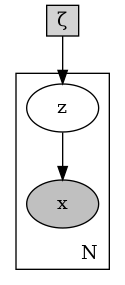
\includegraphics[width=\textwidth]{../plots/vae_p.gv.png}
\caption{generative model ($p(x,z)$}
%\caption{blabla}
%\label{bla}
\end{subfigure}
%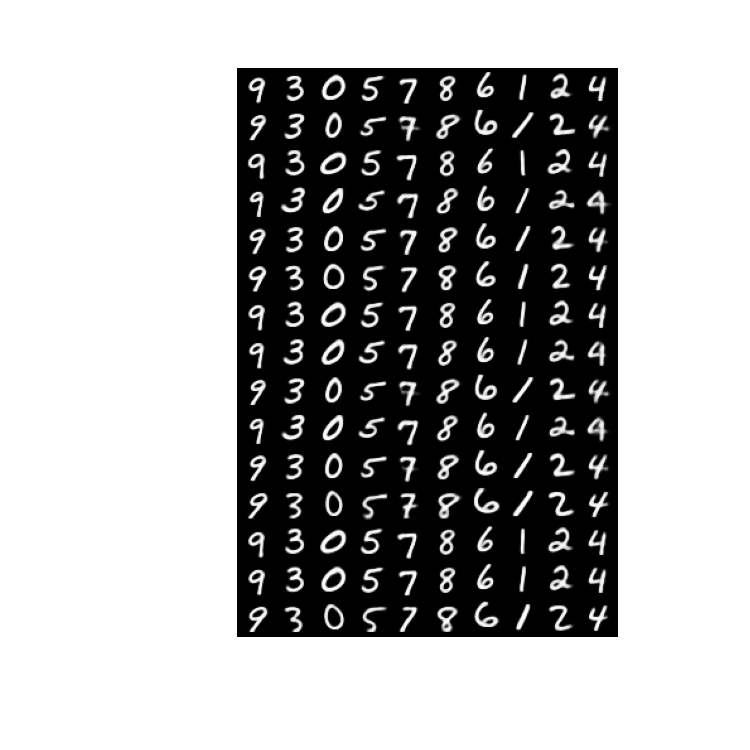
\includegraphics[width=0.4\linewidth]{images/model_mnist_10c_generation.png}
\begin{subfigure}[b]{0.2\textwidth}
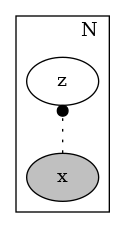
\includegraphics[width=\textwidth]{../plots/vae_q.gv.png}
\caption{inference model ($q(z|x)$)}
%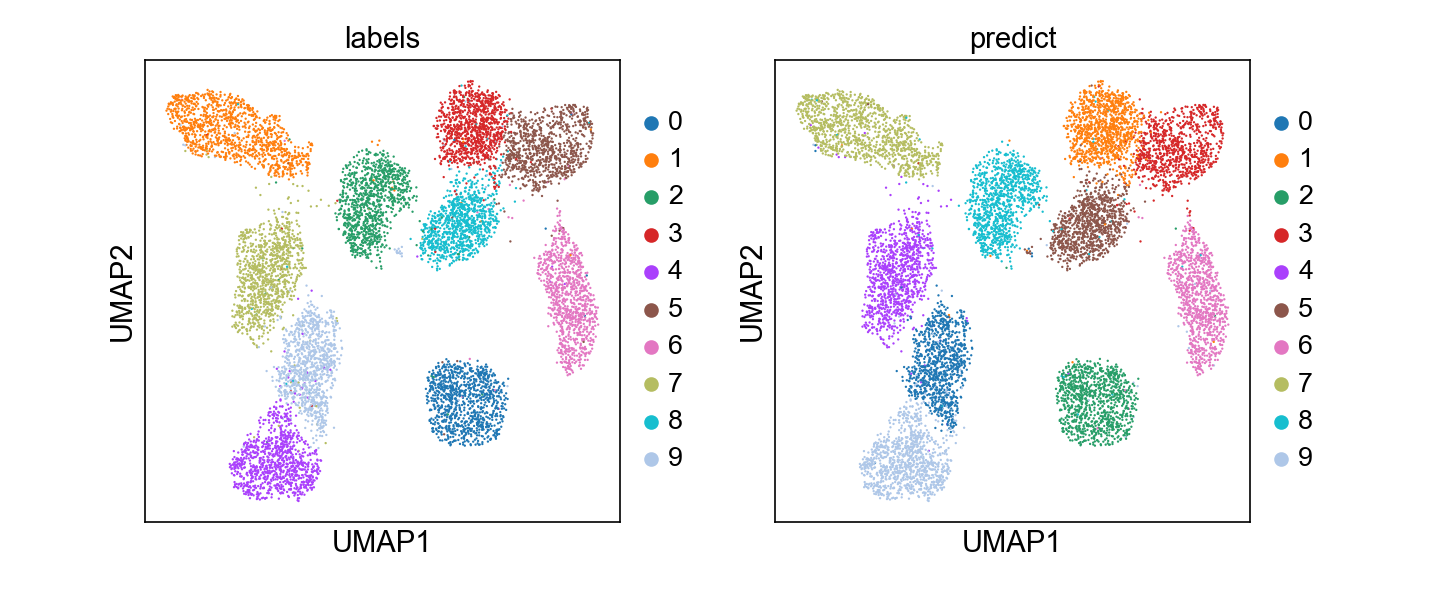
\includegraphics[width=0.4\linewidth]{images/model_mnist_10c_umap.png}
\end{subfigure}
\begin{subfigure}[b]{0.2\textwidth}
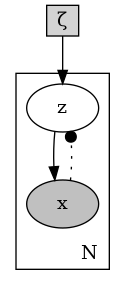
\includegraphics[width=\textwidth]{../plots/vae.gv.png}
\caption{the combined graphical model}
%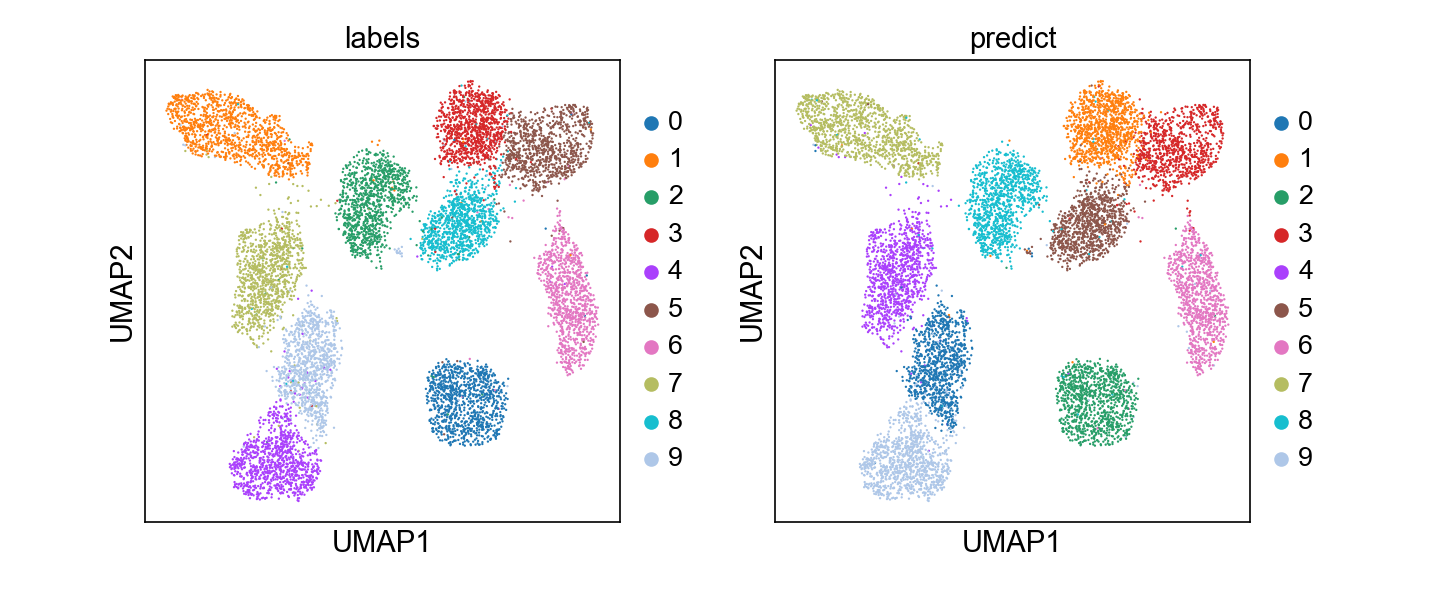
\includegraphics[width=0.4\linewidth]{images/model_mnist_10c_umap.png}
\end{subfigure}
\caption{VAE graphical model}
\label{fig:vae_model}
\end{figure}

Note that the graphical model has no assumption about the specific types of
distributions involved (Gaussian, Dirichlet or whatever \dots) and that is left
for the actual implementation.

In the case of a "vanilla" VAE $(E,D,p)$, 
We use mean field approximation for $p$ and $q$ with Gaussian distributions.
We set the prior $p(\z)$ to be diagonal standard Gaussian
$p(\z) \sim \NN(;\bv{0},\bv{1})$.
And $p(\z | \x) \sim \NN(;D(\z))$ is a diagonal Gaussian, where the decoder
determines its means and variances $D(\z) = (\bv{\mu}(\z), \bv{\sigma}(\z))$, 
And similarly $q(\z | \x) \sim \NN(;E(\x))$.

\section{Expanding the VAE model}
If we look at figure~\ref{fig:vae_model} it looks very simple, but it also
pretty much forces us to choose a simple type of distribution family (e.g
diagonal Gaussians in the case of the vanilla VAE).
Recall that That $\z$ packs up all the latent variables and the stochastic
parameters and $\x$ packs up all the observed variables.

We can describe a more complex distribution by unpacking them and describe the
dependencies between them.
This is done in the following way:
\begin{enumerate}
\item{} define the set of observed random vectors $\x_1, \x_2, \dots \x_k$, and 
the set of latent random vectors and stochastic parameters $\z_1, \dots \z_l$.
\item{} specify how to factor the generative model $p(\x_1,\dots, \x_k| \z_1
\dots , \z_l)$
\item{} specify how to factor the inference model $q(\z_1 \dots \z_l | \x1,
\dots \x_k)$
\item{} choose appropriate priors $p(z_i)$ and
\item{} Chose appropriate distribution families for the $\x_i$ and $\z_i$,
and choose priors $p(\z_i)$.
\end{enumerate}

\subsection{Example: CVAE}
Suppose that we have data that carries both numerical and categorical data $(\X,
C)$.
For example suppose that $\X$ represent a set of images (as flattened vectors),
and $C$ represents the object types shown in the images.
Moreover lets assume that we have $k$ types of categories and that the data is
balanced so we have $k/N$ samples from each category.
We have just specified our observed variables $\x, c$.
We will have one latent variable $\z$ (remember it is actually a vector but we
call them variables...).
The idea here is that because we have different categories, we will have some
type of a mixture of distributions.

Lets specify the generative model $p(\x, \z, c)$. 
We can factor it "arbitrarily" as $p(\x, \z, c) = p(\x | \z, c)p(\z | c)p(c)$.
But we can also simplify if it makes sense. 
Suppose we have reason to believe that $\z$ alone generates
$\x$, so given $\z$, $\x$ and $c$ are treated as independent. But $\z$ itself
will be a mixture of $k$ distributions.
Moreover, since our data is balanced, it is clear that $p(c) = \frac{1}{k}$.
The generative process is therefore as follows:
draw a category $c \sim Cat(\frac{1}{k})$. Then draw $\z \sim p(\z | c)$.
Then draw $\x \sim p(\x | \z)$.
So our factorization of $p$ is:
$p(\x, \z, c) = p(\x | \z)p(\z | c)\frac{1}{k}$.

As for the inference model, given the observation $\x$ and $c$ it will determine
our only latent variable $\z$, in other words $q(\z | \x, c)$ is the inference
model without anything further to factorize.

Now for concrete choice of distribution families:
$p(c)$ is already chosen for us as uniform categorical. 
For the rest we again use diagonal Gaussians.
$p(\z | c)$ will be parametrized by an encoder network taking only the
categorical information. Essentially this network will map each category into
some "blob" around some centroid in the latent space. 
$p(\x | \z)$ describes how given $\z$ it defines a distribution back in the
observed space like the decoder network in the vanilla case.
$q(\z | \x, c)$ means that in this case the encoder takes as input both $\x$ and
$c$ and defines a diagonal gaussian in the latent space.
The difference is that with this model after we train it, the encoder will
encode a mixture distribution in $\z$, we will get several blobs in the latent
space corresponding to the classes.

Remember that the loss function is still the minus elbo but with our
factorization it will become:

\begin{equation}
\begin{aligned}
\label{eq:cvaeloss}
\LL(p,q,\x,c) = 
\int -\log \frac{p(\x,c,\z)}{q(\z | \x, c)}dq \\
= \int -\log \frac{p(\x|\z) p(\z | c) p(c)}{q(\z | \x, c)}dq \\
= \int - \log p(\x | \z)dq + \int \log \frac{q(\z | \x, c)}{p(\z | c)}dq
+ \log(k) \\
= \int - \log p(\x | \z)dq + KL(q(\z | \x, c) \| p(\z | c)) + \text{const}
\end{aligned}
\end{equation}

From equation~\ref{eq:cvaeloss}, we can ignore the constant and we see again a
reconstruction term that will make sure the decoder reconstruct the image in
our example, while the kl-term imposes a mixture distribution in the latent
space.

Finally there are circumstances that we use CVAE to "forget" the categories
rather then to encode them by setting a fixed prior $p(\z | c) \equiv p(\z)$.
An example for such use-case is if we have for example several batches of data,
for the same type of data but from different experiment. In this case we can use
a CVAE model with fixed prior to reduce the batch effect.

%MEMO: add examples with CVAE on MNIST. one with learned prior for mixture
%latent, one with fixed prior for batch effect reduction, one vanilla VAE.
%plots of the umaps...

\chapter{Gaussian mixture model VAEs}

Theoretical background and 
with some examples from publications and my own tests.


\begin{figure}
\centering
\begin{subfigure}[b]{0.4\textwidth}
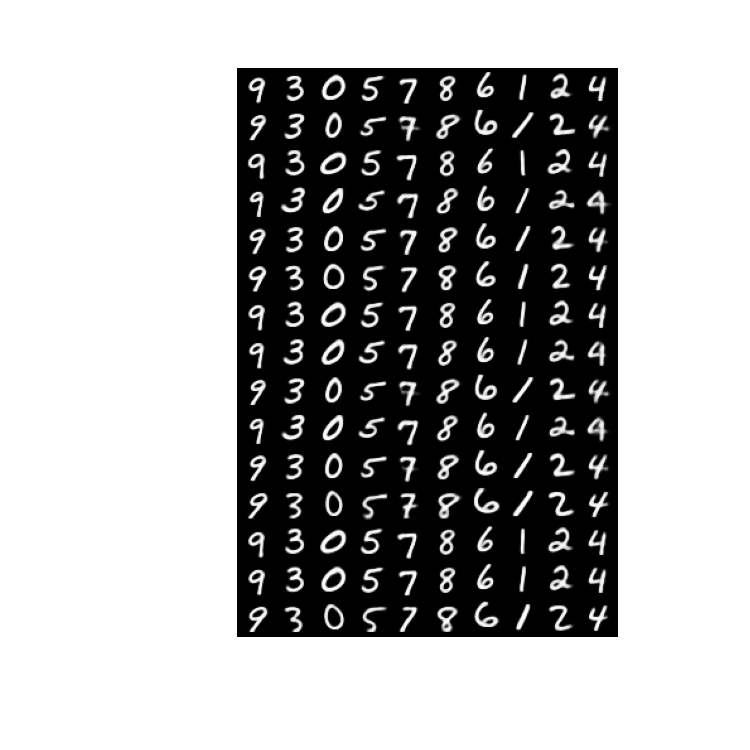
\includegraphics[width=\textwidth]{images/model_mnist_10c_generation.png}
\caption{}
%\caption{blabla}
%\label{bla}
\end{subfigure}
%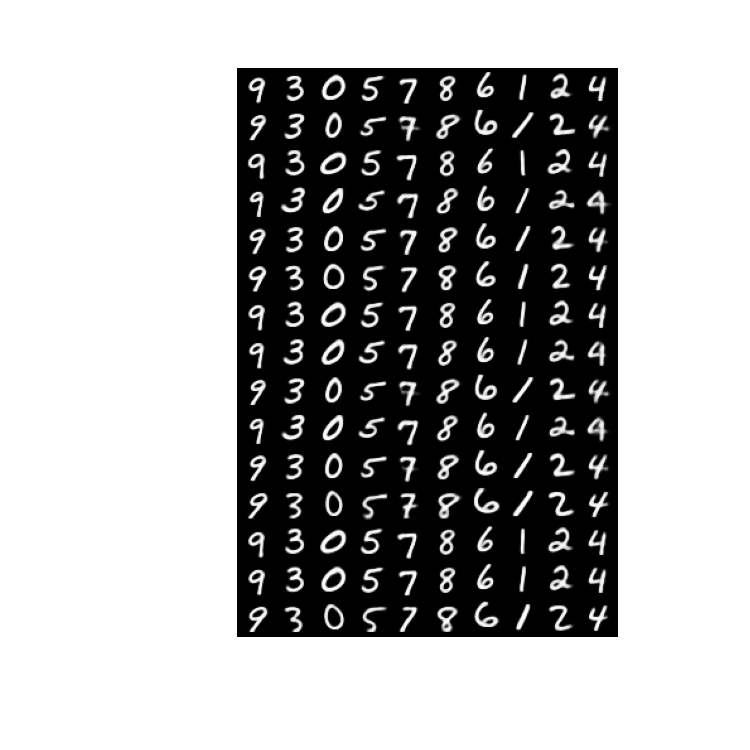
\includegraphics[width=0.4\linewidth]{images/model_mnist_10c_generation.png}
\begin{subfigure}[b]{0.4\textwidth}
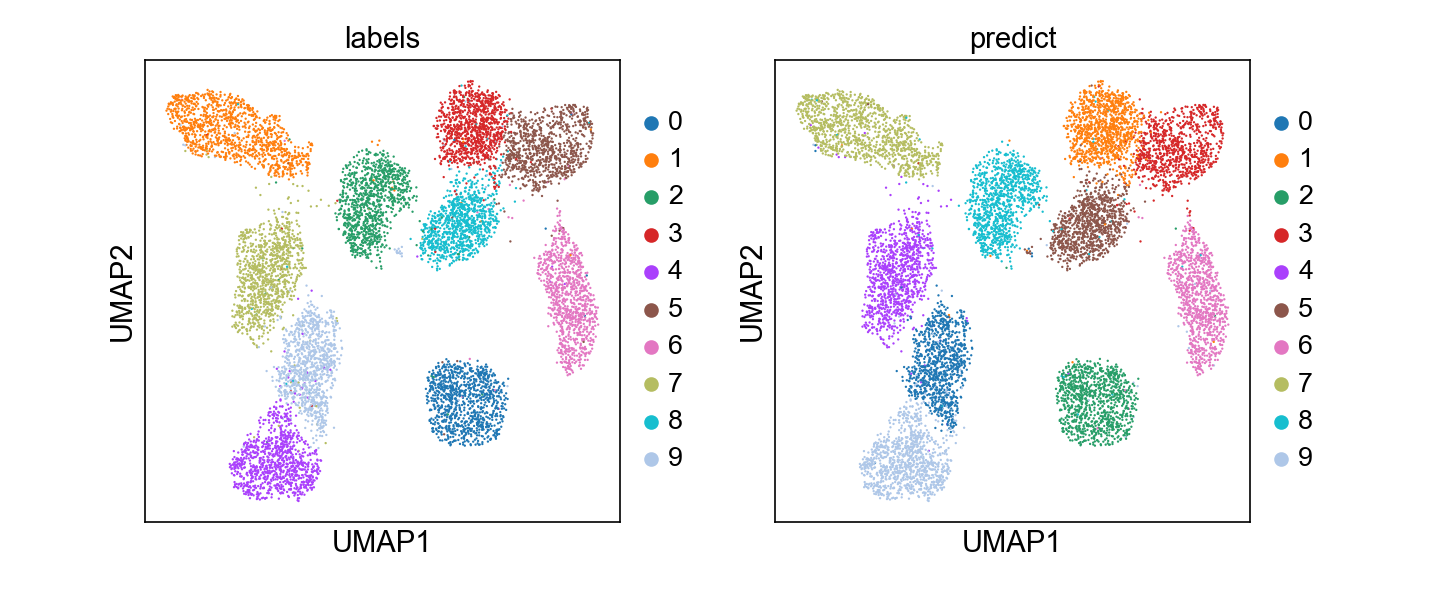
\includegraphics[width=\textwidth]{images/model_mnist_10c_umap.png}
\caption{}
%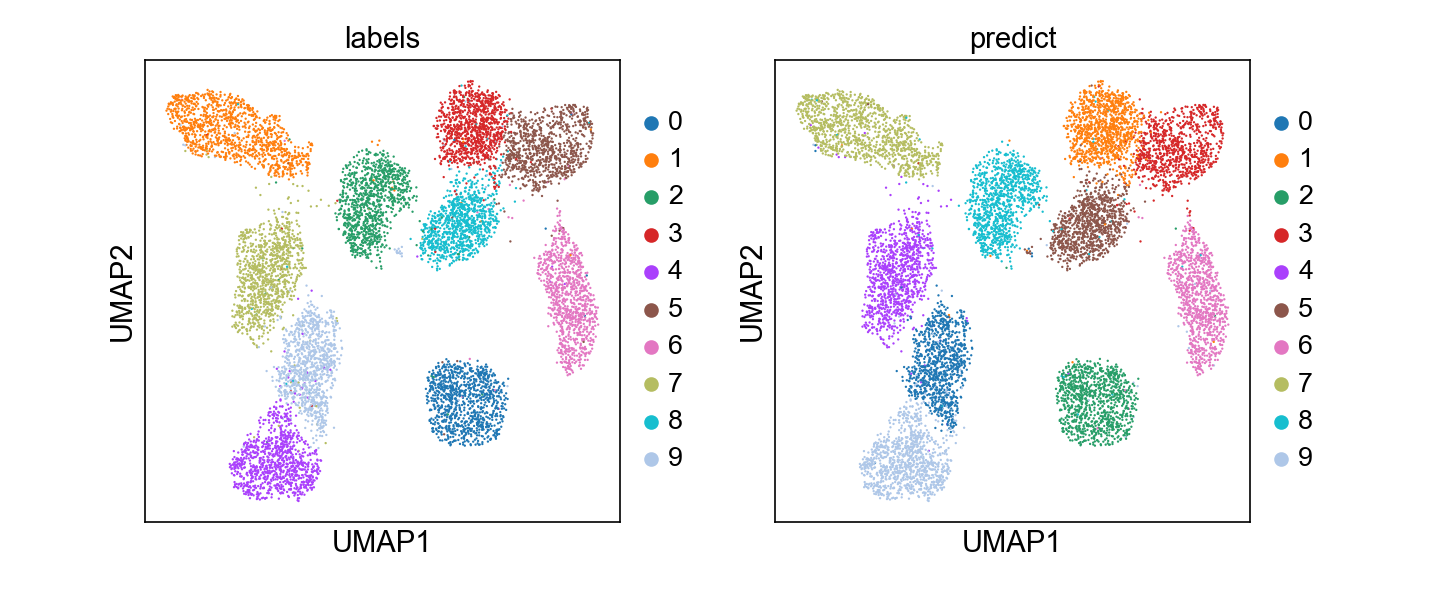
\includegraphics[width=0.4\linewidth]{images/model_mnist_10c_umap.png}
\end{subfigure}
\caption{a figure}
\label{fig:myfig}
\end{figure}

\subsection{Relation between AE and VAE}

\subsection{Conditional VAE}

\chapter{Experiments and results}
\section{Tests with MNIST and FMNIST}

\section{Tests with scRNAseq Data}
some words about (sc)RNAseq and published papers where 
AE and VAE models have been applied.
What we were hoping to achieve and compare with.

\chapter{Discussion, some remarks and conclusions}
punkt.
punkt.
punkt.





%\author{Yiftach Kolb}
%\date{Berlin, \today}
%\maketitle

%\section*{Intro Foo}
%\lipsum{1}
%\section{Bar}
%\lipsum{2}
%\appendix
%\section{Spam}
%\lipsum{3}

\printbibliography

\end{document}


